\documentclass{standalone}
\usepackage{tikz}
\usepackage{bm}

\begin{document}
    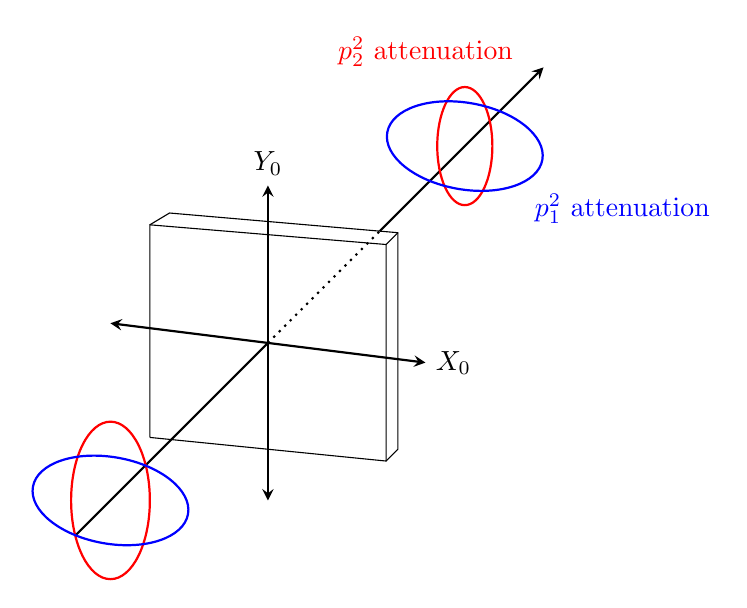
\begin{tikzpicture}[]
        %\draw[step=1cm,gray,very thin] (-2,-2) grid (6,6);
        
        % Axes
        \draw[<->, >=stealth, thick] (-2,0.25) -- (2,-0.25) node[right] {$X_0$};
        \draw[<->, >=stealth, thick] (0,-2) -- (0,2) node[above] {$Y_0$};
        
        % Diattenuator (Brick)
        \draw[] (-1.5,-1.20) -- (1.5,-1.5) -- (1.5,1.25) -- (-1.5,1.5) -- (-1.5,-1.20);
        \draw[] (1.5,-1.5) -- (1.65,-1.35) -- (1.65,1.4) -- (-1.25, 1.65) -- (-1.5,1.5);
        \draw[] (1.65,1.4) -- (1.5,1.25);
        
        % Direction
        \draw[thick] (-2.45,-2.45) -- (0,0);
        \draw[thick, dotted] (0,0) -- (1.42,1.42);
        \draw[thick, ->, >=stealth] (1.42,1.42) -- (3.5,3.5);
        
        % Ellipse before
        \draw[thick, red, rotate around={0:(-2,-2)}] (-2,-2) ellipse (0.5 and 1);
        \draw[thick, blue, rotate around={-10:(-2,-2)}] (-2,-2) ellipse (1 and 0.55);
        
        % Ellipse after
        \draw[thick, red, rotate around={0:(2.5,2.5)}] (2.5,2.5) ellipse (0.35 and 0.75);
        \draw[thick, blue, rotate around={-10:(2.5,2.5)}] (2.5,2.5) ellipse (1 and 0.55);
        
        % Labels
        \draw (4.5, 1.7) node[text=blue] {$p_1^2$ attenuation};
        %\draw[->, >=stealth] (4.5, 1.5) -- (3.5,2.5);
        
        \draw (2, 3.7) node[text=red] {$p_2^2$ attenuation};
        %\draw[->, >=stealth] (4.5, 1) -- (3.5,2.5);
        
        
    \end{tikzpicture}
\end{document}